\subsubsection{Minuta de reunião (12-Novembro-2015)}

\begin{tabbing}
  Local \= xxx \kill
  Local \> : LEAD \\
  Data  \> : 12 de Novembro de 2015 \\
  Hora  \> : 13:00
\end{tabbing} 

%---------------------------------------------------------------------
\participantes{
  \gabriel,
  \julia,
  \estevão,
  \elael,
  \renan,
  \ramon.

}

\textbf{Aprovação da minuta}

\textbf{Update semanal do Projeto EMMA} 

\text {Objetivo para conclusão da viabilidade técnica}
   									
					
		
		\item \textbf{Pá 1:1}
			\begin{itemize} 
			    \item Design e construção.
			\end{itemize}
			
		\item \textbf{Manipulador}
			\begin{itemize} 
			    \item Definir controle através do ROSS ou do ROCK.
			    \item Telemetria
			    \item Software: Move it ou Planning
			\end{itemize}	

		\item \textbf{Pintura\Coating}
			\begin{itemize} 
			    \item Definir 'atuador' que fará a simulação do metalização..
			\end{itemize}	
		
		\item \textbf{Scanner}
			\begin{itemize} 
			    \item Extrair dados da pá para  ROCK e para o ROSS, pacotes de
			    desenvolvimento utlizados na área de robótica.
			    \item Alinhamento das medidas dos modelos extraídos com oclusão.
			    \item Dados do braço robótico.
			    \item Teste de calibração esquematizado.
			\end{itemize}
			
				
\item \textbf{Requisitos para espaço destinado a teste}
			\begin{itemize} 
			    \item Preço estimado para:
			    \item Pá (estevão)
			    \item manipulador (orçamento)
				\item pistola de tinta 
				\item trilhos (estevão)
				\item scanner (gabriel)
				\item base (estevão)
				\item infraestrutura
   				\item restrições apresentar projeto para arquiteta da Coppe
   			\end{itemize}	




\textbf{Agenda para a próxima reunião:}
  \begin{itemize}
    \item Resultado de pesquisas individuais.
    \item Novas tarefas \& recomendações.
  \end{itemize}


\vspace{5mm}%
\parbox[t]{70mm}{
  Aprovado por: \\[5mm]
  \centering
  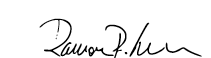
\includegraphics[width=65mm]{figs/logo/assinatura-ramon.png} \\[-4mm]
  \rule[2mm]{70mm}{0.1mm} \\
  \ramon \\[1mm]
  Coordenador do Projeto \\
}

%---------------------------------------------------------------------
\fim